\documentclass[11pt,letterpaper,oneside]{report}
\usepackage[margin=1in,footskip=0.42in]{geometry}
\usepackage[T1]{fontenc}
\usepackage{helvet}
\usepackage{graphicx,booktabs,tabularx,array,caption,xcolor,listings,amsmath}
\usepackage[hidelinks]{hyperref}
\renewcommand{\familydefault}{\sfdefault}
\renewcommand{\contentsname}{Table of Contents}
\setlength{\parindent}{0pt}
\setlength{\parskip}{.65em}
\setlength{\emergencystretch}{2em}
\linespread{1.17}
\setcounter{tocdepth}{1}
\graphicspath{{assets/}}
\captionsetup{font=small,labelfont=bf}
\definecolor{ink}{HTML}{1B3441}
\definecolor{papergray}{HTML}{F3F5F7}
\definecolor{good}{HTML}{21694C}
\definecolor{warn}{HTML}{9C4934}
\lstset{basicstyle=\ttfamily\small,backgroundcolor=\color{papergray},frame=single,rulecolor=\color{black!18},columns=fullflexible,breaklines=true,keepspaces=true,showstringspaces=false,framexleftmargin=4pt}
\hypersetup{pdftitle={SentinelAPI - Information Security Project Report},
  pdfauthor={Soham Agarwal, Aayush Doshi, Divyam Khandelwal, Prem Sharma}}
\makeatletter
\renewcommand{\@makechapterhead}[1]{%
  {\centering\parindent\z@\normalfont\Large\bfseries
    Chapter \thechapter: #1\par\nobreak\vskip 18pt}}
\renewcommand{\@makeschapterhead}[1]{%
  {\centering\parindent\z@\normalfont\Large\bfseries #1\par\nobreak\vskip 18pt}}
\makeatother
\newcommand{\ProjectTitle}{SentinelAPI}
\newcommand{\ProjectSubtitle}{Local API Intrusion Detection and Security Playground}
\newcommand{\Course}{IT305 Information Security}
\newcommand{\Supervisor}{Dr Pooja Mishra}
\newcommand{\AcademicYear}{2026--27}
\newcommand{\Institute}{Indian Institute of Information Technology Vadodara}
\newcommand{\Department}{Department of CSE}
\newcommand{\TeamRows}{Soham Agarwal & 202452332\\Aayush Doshi & 202452301\\Divyam Khandelwal & 202452316\\Prem Sharma & 202452328\\}
\newcommand{\topic}[1]{\smallskip\noindent\textbf{#1}\par\nobreak\vspace{-.39em}}
\newcommand{\casecode}[1]{\texttt{#1}}
\newcommand{\sheet}[1]{\clearpage\section{#1}}
\newcommand{\tabletitle}[1]{\captionof{table}{#1}\smallskip}
\newcolumntype{Y}{>{\raggedright\arraybackslash}X}
\newcommand{\bodytable}[1]{\begin{tabularx}{\linewidth}{@{}>{\raggedright\arraybackslash}p{.25\linewidth}Y@{}}\toprule #1\bottomrule\end{tabularx}}
\newcommand{\callout}[1]{\noindent\colorbox{papergray}{\parbox{\dimexpr\linewidth-2\fboxsep\relax}{\small\strut #1\strut}}}
\newcommand{\diagram}[1]{\begin{center}\footnotesize #1\end{center}}
\newcommand{\nodebox}[1]{\fbox{\strut #1}}
\newcommand{\arr}{\ \(\longrightarrow\)\ }
\begin{document}
\pagenumbering{gobble}
\begin{titlepage}
\centering
\vspace*{.30in}
\begin{minipage}{.22\textwidth}
  \centering
\includegraphics[width=\linewidth,trim=150 150 150 150,clip]{iiitlogo.png}
\end{minipage}\hspace{.17in}%
\begin{minipage}{.60\textwidth}
  \raggedright\Large\bfseries \Institute
\end{minipage}

\vspace{.62in}
{\Large\bfseries\underline{Information Security Project Report}\par}
\vspace{.24in}
{\LARGE\bfseries\ProjectTitle\par}
\vspace{.08in}
{\large\bfseries\ProjectSubtitle\par}
\vspace{.30in}
{\large\bfseries\Course\par}
\vspace{.20in}
{\large\bfseries \Department\\Academic Year \AcademicYear\par}

\vspace{.52in}
\begin{minipage}[t]{.59\linewidth}
\raggedright\textbf{Submitted By}\par\smallskip
\begin{tabular}{@{}ll@{}}\TeamRows\end{tabular}
\end{minipage}%
\begin{minipage}[t]{.40\linewidth}
\centering\textbf{Under the Guidance of}\par\smallskip
\Supervisor
\end{minipage}
\vfill
\rule{.83\textwidth}{.5pt}
\end{titlepage}

\pagenumbering{roman}
\chapter*{CERTIFICATE}
This certificate accompanies the project report entitled \emph{\ProjectTitle: \ProjectSubtitle}, submitted by the following students of \Institute\ (IIITV) as part of the academic requirements for \Course\ in the academic year \AcademicYear.

The supervisor's signature below records approval of the submission. The report describes the work undertaken by the team and identifies the references and external resources used.

\bigskip
\textbf{Project Title}\quad \ProjectTitle: \ProjectSubtitle

\textbf{Group Number}\quad\rule{2.35in}{.4pt}

\bigskip
\textbf{Team Members}
\begin{center}
\begin{tabular}{@{}p{.51\linewidth}p{.26\linewidth}@{}}
\toprule
\textbf{Name} & \textbf{Roll Number}\\
\midrule
\TeamRows
\bottomrule
\end{tabular}
\end{center}
\bigskip
\textbf{Project Supervisor}\quad \Supervisor

\vspace{.75in}
\textbf{Signature of Supervisor}\quad\rule{2.3in}{.4pt}

\textbf{Date}\quad\rule{2.3in}{.4pt}

\chapter*{Abstract}
\phantomsection\addcontentsline{toc}{chapter}{Abstract}
SentinelAPI is a local information security laboratory that connects application-layer request inspection with a repeatable method for evaluating defenses. An Express middleware examines selected HTTP inputs using seven signature-based checks and four behavioral checks. A React dashboard lets authorized users run experiments, examine each response, inspect the rules and counters behind a decision, and review related incidents. PostgreSQL keeps run results, alerts, and investigation records. The laboratory uses signatures and explicit thresholds throughout.

Each test case specifies an expected HTTP response and, where applicable, an expected detector alert. The simulator sends actual requests to an authenticated local API and checks the response against the associated database evidence. Demonstration endpoints return controlled responses and treat submitted input as data. The full Standard suite has 175 checks. A saved Standard run matched all expectations, with 62 HTTP~200, 8 HTTP~401, 78 HTTP~403, 15 HTTP~404, and 12 HTTP~429 responses. A separate Extended SQL and XSS run matched 106 of 142 expectations, identifying 36 missing expected detector attributions. A later normal-traffic check passed all 12 controls.

The Defense Lab compares an intentionally broad practice rule against the current SQL signature on 21 labeled cases. The specific rule improved six decisions, including accepting a legitimate name containing an apostrophe, with zero regressions on this set. Incident timelines connect alerts and analyst actions. A keyed audit chain verifies newly signed events and detects edits or a missing tail in a disposable sample. The latest implementation check passed 12 automated tests. Results apply to the tested laboratory cases and document where the defenses need broader evaluation.

\textbf{Keywords:} application-layer intrusion detection, API security, signature matching, rate limiting, false positives, incident triage, tamper-evident audit.

\tableofcontents
\clearpage
\pagenumbering{arabic}

\chapter{Introduction}
\section{Background and Context}
Web APIs accept data through URLs, request bodies, headers, uploaded files, and repeated interactions. A syntactically valid request can still carry input that resembles an injection attempt or form part of abusive behavior. Conversely, ordinary text can resemble a suspicious pattern when interpreted without context. A search for a family name with an apostrophe is a useful illustration of why a broad signature can interfere with normal work.

Intrusion detection records evidence that a condition was met. Intrusion prevention changes the outcome of the request, for example by rejecting the request before a handler runs. NIST describes both functions in its guide to intrusion detection and prevention systems \cite{nist}. SentinelAPI applies the distinction at the HTTP application layer. It can record a missing-route pattern without changing a 404 response, enforce a temporary rate limit with 429, or actively block a signature match with 403.

The project combines a protective middleware, a closed laboratory, and an analyst interface. The browser configures an experiment and shows the resulting evidence. The server creates the cases, sends them to its own API, checks the responses, and stores the results. This arrangement makes it possible to follow the full path from submitted input to an analyst's decision about an alert.

\topic{Why the application layer matters}
The middleware operates on parsed HTTP data. It sees a field name, a body value, a header, an uploaded file buffer, or a count associated with a request scope. This view makes rules understandable in terms of application behavior. The project consequently evaluates API request handling rather than packet inspection or network-flow classification.

\topic{Information security goals}
Confidentiality motivates the checks related to unauthorized database, file, and internal-service access. Integrity motivates the checks for unexpected database or command behavior and the audit verification feature. Availability motivates measuring a short burst, the temporary limit, and recovery. Each goal is represented by a test or a recorded event that can be examined during the demonstration.

\sheet{Problem Statement, Aim and Objectives}
\topic{Problem statement}
How can a local API security laboratory show whether a rule correctly detected a suspicious request, allowed a legitimate request, and recorded enough evidence to justify the outcome? A status code alone gives an incomplete answer. A 403 could be an authorization decision or the result of a particular detector. Likewise, a 404 can be the expected application response even when repeated missing routes have produced a security alert.

\topic{Aim}
Design and evaluate a rule-based API security laboratory in which request decisions are observable, experiments are repeatable, and analyst actions can be audited.

\topic{Objectives}
\begin{enumerate}
\item Inspect selected query, body, header, path, and upload inputs before application processing.
\item Track selected behavioral patterns within bounded time windows.
\item Provide controlled experiments with suspicious cases and normal-traffic controls.
\item Compare the actual response and persisted detector identity with the expected result for each case.
\item Explain decisions using a rule identifier, the inspected field, and measured counters where available.
\item Support incident review and verification of newly signed audit events.
\end{enumerate}

\topic{Acceptance example}
A normal search that returns 200 with no linked alert meets its expected result. A signature case that returns 403 reaches its expected result only when the required detector also has a linked record. A threshold-based case can have different expected results at different points in its sequence. Together these conditions allow a reviewer to distinguish a block, an ordinary rejection, an unexpected detector, and a missing detector.

\callout{The unit of evaluation is a defined test case with explicit expectations. Each expectation is interpreted in the context of the scenario and its position in the sequence.}

\sheet{Significance, Scope and Report Organisation}
The technical contribution is an evidence workflow spanning detection, testing, and investigation. A student can start with a case, inspect what the server measured, compare a rule change on the same labeled inputs, and then see how an alert was handled. This makes it possible to discuss both a successful rule match and a false positive using concrete evidence.

\tabletitle{Scope of the project}
\bodytable{\textbf{Area} & \textbf{Included work}\\\midrule
Inspection & HTTP request signatures and short behavioral windows.\\
Experimentation & Predefined local scenarios, normal controls, Extended inputs, and selected custom inputs.\\
Analyst workflow & Alert states, review verdicts, incident timelines, role and ownership restrictions.\\
Evidence & Saved experiment results, exports, audit records, and verification for signed events.\\
Evaluation & Recorded lab runs, a fixed comparison set, automated tests, and isolated database checks.\\}
\par

Several features have deliberately limited claims. The lab handlers keep submitted SQL, scripts, and shell text inert and simulate fetch behavior. The request-flood scenario measures single-host HTTP behavior and recovery. Counters operate in one backend process. The audit verifier assumes access to the signing key remains controlled and the checkpoint has not been rolled back with the entire database.

\topic{Organisation of the report}
Chapter 2 reviews intrusion detection, web security testing, and audit evidence. Chapter 3 presents the architecture, data flow, state, and decision semantics. Chapter 4 describes the stack, setup, and test data. Chapter 5 explains the implementation and detector families with code samples. Chapter 6 defines tests and metrics. Chapter 7 reports observed outcomes and interprets differences between profiles. Chapter 8 concludes with limitations and future work.

\chapter{Literature Review}
\section{Signature and Behavior-Based Detection}
Intrusion detection systems collect and interpret evidence about potentially unwanted activity. Scarfone and Mell discuss signature-based detection, anomaly-based detection, and stateful protocol analysis in the context of IDPS technologies \cite{nist}. These categories are useful for this project because the same API uses rules that evaluate one input and rules that require a short history.

A signature specifies an observable pattern. It can be reviewed by a student and linked directly to an explanation. For example, the report can identify a request field and state that a SQL-like construct matched a specific rule. The explanation supports auditing, but its specificity does not establish the probability of compromise. A match reports the presence of a selected pattern under the laboratory's parsing rules.

Behavioral checks reduce individual events to a defined measure. Selecting the scope and window is as important as selecting the threshold. A count by source and username answers a different question from a count of distinct usernames associated with one password group. The thresholds used in this project are selected for demonstration and evaluation on fixtures.

\topic{Relationship to learning-based systems}
An anomaly model may learn a statistical profile from historical observations. SentinelAPI uses explicit windows and limits that can be shown directly in the dashboard. Its training-free design means that each result can be traced to a rule or counter without a training dataset. The trade-off is that quality depends on the chosen signatures and on whether the test inputs represent the expected request context.

\tabletitle{Two sources of detection evidence}
\bodytable{\textbf{Mechanism} & \textbf{Example evidence}\\\midrule
Signature & Name of the rule and the field or file element it evaluated.\\
Behavior & Measured count, threshold, observation window, and resulting HTTP decision.\\}

\sheet{Web Security Testing and Case Design}
The OWASP Web Security Testing Guide separates areas such as authentication, authorization, session management, and input validation \cite{owasp}. This helps structure the evaluation. A failed login is useful for validating authentication behavior, while a separate access-control test checks whether one authenticated user can retrieve another user's run. Combining these observations into one count would hide what each control achieved.

Bozic and Wotawa propose planning-based testing using attack grammars to connect test sequences and concrete inputs \cite{bozic}. Their approach is relevant to the distinction between describing a scenario and executing it. SentinelAPI keeps that distinction in its catalog and runner. The catalog defines a fixed local plan and expected outcomes, while the runner performs the requests and checks evidence. Tests do not require an external target, a planner, or generated attack workflows.

A test oracle determines what counts as a successful test. In SentinelAPI the oracle can check a response, look for the required detector, and require the absence of an alert for a benign case. This is stronger than visual judgment based on response color. It also makes the result sensitive to which detector fired. If another rule blocks an input, the expected detector can still be missing.

\topic{Positive and negative controls}
Positive controls establish whether recognizable suspicious input or behavior is detected. Negative controls establish whether valid input continues to work. A meaningful comparison must use the same cases for both rules and hold the expectations constant. The comparison of an apostrophe-only practice rule with the current SQL signature follows this approach.

\topic{Repeatability}
The selected profile, case counts, local endpoints, run identifiers, and artifact timestamps constrain interpretation. When a scenario depends on timing, the test design must identify the relevant phase and verify recovery separately from merely seeing a rejection.

\sheet{Alert Investigation and Evidence Integrity}
Detection is only the start of an investigation. An alert can be reviewed, confirmed, marked as a false positive, or left pending. The outcome of that judgment is different from the workflow state of the alert. An alert can be resolved after a false-positive review, and the final state should still preserve the analyst's finding.

Logs support accountability when they retain sufficient context and can be read in sequence. SentinelAPI groups detections and investigator actions by experiment so a reviewer can see when a run started, which alerts were emitted, and which changes followed. The grouping key is the run identifier, and the result is an investigation aid for experiments with linked alerts.

The integrity design uses HMAC as described by Krawczyk, Bellare, and Canetti \cite{hmac}. Each event is authenticated using a value derived from the event and its predecessor. A signed checkpoint commits to the tail and expected count. When a verifier recomputes the chain, changing an event changes that event's expected tag. Removing the final event leaves the remaining chain with a different tail or count from the checkpoint.

\tabletitle{Security decisions and evidence decisions}
\bodytable{\textbf{Decision} & \textbf{Question answered}\\\midrule
Request outcome & Did the API allow, reject, rate limit, or report the request?\\
Expectation outcome & Did this result meet the criteria specified by the case?\\
Analyst verdict & Does a reviewer consider the alert a confirmed detection or a false positive?\\
Audit integrity & Do the signed records match the saved checkpoint?\\}

Cryptographic verification depends on protecting the secret and retaining a trustworthy checkpoint. It does not label an analyst's verdict as correct. It verifies the recorded sequence within the selected signed range, including whether the records still agree with the chain produced by the application.

\sheet{Related Work, Research Gap and Project Justification}
Different security systems answer different questions. A network IDPS monitors traffic at a network observation point. A web security testing methodology gives coverage categories and verification practices. A planning-based research system generates test sequences. SentinelAPI connects a smaller set of controlled API experiments with the evidence that a human reviewer needs to understand what happened.

\tabletitle{Relationship between references and project design}
\bodytable{\textbf{Reference} & \textbf{Relationship to SentinelAPI}\\\midrule
NIST IDPS guide \cite{nist} & Provides a framework for distinguishing detection and prevention. SentinelAPI applies the distinction at the HTTP application boundary.\\
OWASP WSTG \cite{owasp} & Helps separate input handling, authentication, and authorization tests.\\
Bozic and Wotawa \cite{bozic} & Motivates separating test descriptions from concrete execution and observations.\\
HTTP specifications \cite{http,rfc429} & Explain response semantics used when measuring and labeling outcomes.\\
HMAC specification \cite{hmac} & Supports the keyed authentication mechanism used for audit integrity verification.\\}

\topic{Project gap}
A small academic demonstration can show a detection without explaining whether normal requests are safe or why a particular rule matched. SentinelAPI addresses that gap by placing a fixed rule comparison, individual request evidence, and investigation actions alongside the detection catalog. The contribution is the integration and reproducible demonstration of these components.

\topic{Evaluation question}
The report evaluates whether the middleware and investigation workflow behave as implemented. Results come from locally saved traffic, a fixed comparison dataset, and targeted verification checks. The findings do not estimate enterprise detection rates or operational workload under real traffic distributions.


\chapter{Methodology and System Design}
\section{Proposed Framework}
The architecture has five cooperating parts. The presentation layer holds the dashboard and terminal client. The API authenticates users and exposes management and protected routes. The experiment service constructs and executes a bounded case plan. Middleware evaluates each protected request before it reaches a lab handler. PostgreSQL stores results, alerts, users, and investigation events.

\diagram{\nodebox{Dashboard or CLI}\arr\nodebox{Authenticated API}\arr\nodebox{Experiment worker}\\[8pt]
\nodebox{Loopback request}\arr\nodebox{Detector pipeline}\arr\nodebox{Controlled handler}\\[8pt]
\nodebox{HTTP response}\arr\nodebox{Verifier and database}\arr\nodebox{Result view}}
\captionof{figure}{SentinelAPI experiment architecture. Management calls and loopback test requests serve separate roles.}

\tabletitle{Major components and their responsibilities}
\bodytable{\textbf{Component} & \textbf{Responsibility}\\\midrule
React interface & Configure a scenario, inspect decision evidence, and navigate results.\\
Express API & Authenticate, validate options, dispatch routes, and return status.\\
Runner and catalog & Produce labeled cases, bind requests to a run, and verify the evidence.\\
Detector middleware & Inspect inputs and counters and make request-level decisions.\\
PostgreSQL & Persist account, run, alert, review, and audit information.\\}

A protected lab request passes through the same middleware regardless of whether an authenticated user or the controlled simulator initiated it. Simulator metadata is accepted only when associated with a registered active case and its owner. This lets investigators trace results to the correct experiment without allowing arbitrary headers to select a new state bucket.

\sheet{Request, Decision and Evidence Lifecycle}
The system has a control path and a data path. The control path handles sign-in, configuration, start, poll, cancel, and report requests. The data path carries the experiment's individual HTTP requests. They are tagged with the active run and case identifiers so that detector alerts can later be located. That association is checked at the middleware boundary.

\begin{enumerate}
\item The operator selects a scenario, profile, and optional settings in the playground.
\item The API evaluates role and configuration constraints and creates a run record.
\item The runner sends each defined case to the local API.
\item Middleware checks whether the request is in an active rate-limit window and applies the detectors in order.
\item The runner captures the actual response and reads the database evidence attributed to the case.
\item The verifier compares the observations with the expectation. The report is updated with progress and final state.
\end{enumerate}

\topic{Three independent observations}
A blocked request has an HTTP result. A detector alert has an identity, reason, and severity. A test has a result based on its declared expectations. For example, an HTTP~404 is the normal result for a nonexistent route. The same response can also meet the expectation for an enumeration threshold when the relevant alert is present.

\topic{Live alerts and saved evidence}
The event stream notifies the dashboard when relevant alert data changes. A run report is stored independently of the live connection. On reopening a report, the UI reads the saved evidence. The replay feature moves through those rows without sending the requests again.

\callout{A result can be reconstructed from the response status, required detector, and linked alert IDs. A color or result badge alone is insufficient evidence.}

\sheet{Trust Boundaries and State Isolation}
\topic{Authentication boundary}
The dashboard account and the demo login route have different functions. Account sign-in uses database-backed credentials. The demo route provides a controlled response for login-behavior scenarios. A request to the demo route still needs to cross the application boundary with an authenticated operator identity.

\topic{Evidence ownership boundary}
Roles define permitted actions. Object ownership is checked separately so that knowing another run or alert identifier is insufficient to read or modify it. An administrator can review global evidence. An analyst can work with owned records, and a viewer has read access to owned records. The comparisons use a fixed shared set of labeled cases.

\topic{Detector state boundary}
Ordinary request state is scoped by authenticated user and source. For simulator traffic, state is isolated by run and case lane. A lane groups the requests that together form a behavioral experiment, such as successive failures for one account. Completion or cancellation releases temporary simulation state. This arrangement helps avoid cross-scenario effects, such as a request burst changing the result of a separate login scenario.

\tabletitle{Evidence preserved at each boundary}
\bodytable{\textbf{Boundary} & \textbf{Evidence or validation}\\\midrule
Account & Credential verification and an active user record.\\
Run and case & Valid active run, correct owner, known case identity.\\
Alert review & Current role, alert ownership, saved verdict, audit event.\\
Audit chain & Recomputed tag, checkpoint signature, expected event count.\\}

\topic{Persistence boundary}
Counts and temporary limits remain in process memory. Alerts, reports, and review verdicts survive a restart through PostgreSQL. A restart can leave a run incomplete, so persisted progress remains useful even if the remaining requests were never executed.

\sheet{Algorithms and HTTP Decision Semantics}
\tabletitle{Interpretation of HTTP outcomes within the lab}
\begin{tabularx}{\linewidth}{@{}lXX@{}}\toprule
\textbf{HTTP} & \textbf{Typical observation} & \textbf{Evidence interpretation}\\\midrule
200 & A controlled handler accepts a request. & A normal control expects no alert.\\
401 & Demo credentials are invalid. & An early failed attempt can meet its expectation.\\
403 & A request is refused. & The required detector record confirms an expected signature or behavior block.\\
404 & The requested lab route does not exist. & Repeated 404s can have an enumeration alert at the threshold.\\
429 & The request rate is limited. & A recorded threshold event explains the active cooldown.\\
503 & Inspection cannot be completed. & A service problem calls for investigation, not classification.\\
\bottomrule\end{tabularx}

HTTP status meanings follow the protocol semantics \cite{http,rfc429}. Scenario-specific interpretations depend on the context above. Management routes may also use these codes for their own authentication, access, or service decisions.

\topic{Signature checks}
The application extracts string values from selected request locations and normalizes common encodings before pattern matching. Field paths can be attached to a decision. Sensitive values are redacted in the structured matched-input evidence.

\topic{Behavioral checks}
A detector keeps recent timestamps or distinct identities for a specific scope. It discards observations outside the window. Reaching a threshold can emit an alert, block the current request, or set a cooldown depending on the rule.

\topic{Audit verification}
Audit events are ordered by database record ID. The verifier recomputes each authentication tag and then compares the final tag and count with a signed checkpoint. Verification is an administrative operation. The standalone demonstration changes a temporary copy of signed records.

\chapter{Tools and Technologies}
\section{Programming Languages, Frameworks and Libraries}
TypeScript is used across the backend, the dashboard, and the shared contracts. This lets request results and decision evidence use common field names between components. The runtime still verifies untrusted inputs because TypeScript annotations are removed during execution.

\tabletitle{Technologies and their roles}
\bodytable{\textbf{Technology} & \textbf{Role in the project}\\\midrule
Node.js and TypeScript & API execution, local client, shared data contracts, and automated tests.\\
Express & HTTP routing and input/detection middleware.\\
React and Vite & Dashboard state, navigation, inspection views, development server, and build.\\
PostgreSQL and \casecode{pg} & Persistent accounts, reports, alerts, reviews, and integrity checkpoint.\\
bcryptjs & Password hashing and verification.\\
jsonwebtoken & JWT creation and validation.\\
Multer & Multipart decoding and in-memory file buffers for upload inspection.\\
Node test and assert & Automated checks for detectors, reports, comparison, and audit integrity.\\
Oxlint & Frontend linting.\\}

\topic{Why this stack fits the project}
A single application language is convenient for tracing evidence from detector to dashboard. PostgreSQL provides durable records, transactions, and scoped queries. Vite separates the local UI development loop from server logic. The simulator can verify the API by reading the same HTTP results and stored records relevant to a normal investigation.

\topic{Version reproducibility}
Use the repository's lockfiles when installing dependencies. The report's result tables identify the run artifacts used as evidence. Dependency installation and package versions can differ between machines, so repeat the verification checks after installing in a new environment.

\sheet{Software, Hardware and Local Setup}
The project is intended for a developer laptop with a current browser, Node.js 22 or later, npm, and PostgreSQL 14 or later. The documented macOS setup uses PostgreSQL 16. A single machine is sufficient for the API, dashboard, and test runner. Hardware figures in this report are setup considerations rather than measured capacity limits.

\tabletitle{Local components and configuration}
\bodytable{\textbf{Component} & \textbf{Default or purpose}\\\midrule
API & \texttt{http://localhost:3000}; handles local HTTP and database work.\\
Dashboard & \texttt{http://localhost:5173}; connects through a configurable API URL.\\
Database & PostgreSQL with local database \texttt{sentinelapi}; configuration via \texttt{DATABASE\_URL}.\\
Frontend origin & Must agree with the URL used by the browser for cookies and live updates.\\
Audit key & Set \texttt{AUDIT\_INTEGRITY\_SECRET} before signing begins, or use the configured local fallback. Keep the original signing key available.\\}

\begin{lstlisting}[caption={Setup and verification commands from the repository root}]
npm ci
npm ci --prefix dashboard
npm run check

# Terminal 1, with PostgreSQL available
npm run dev

# Terminal 2
cd dashboard
npm run dev -- --host localhost --strictPort
\end{lstlisting}

The database must exist before starting the API on a fresh installation. The server adds its tables, indexes, and additive schema updates during startup. A health request verifies both server reachability and database connectivity. Existing data and configured local secrets should be retained between restarts.

\sheet{Test Inputs, Provenance and Profiles}
The Standard profile contains project-defined suspicious inputs and ordinary traffic. Each line of evaluation is linked to a defined scenario and may specify a response code, detector, or absence of an alert. A separate set of community inputs broadens SQL and XSS coverage in the Extended profile.

\tabletitle{Test sets and their composition}
\bodytable{\textbf{Set} & \textbf{Composition}\\\midrule
Standard & 175 HTTP requests with the default 20 demo password attempts and all scenarios selected.\\
Full Extended & 295 planned HTTP requests, including 120 additional SQL and XSS probes.\\
Selected Extended & 142 SQL and XSS requests in the recorded two-family run.\\
Rule comparison & 21 fixed search fixtures evaluated offline by two rule definitions.\\
Normal traffic & 12 HTTP requests covering routine search, upload, login, and simulated fetch behavior.\\}

The community corpus is bundled from SecLists \cite{seclists}. The repository records the pinned revision, attribution, and license information. The bundled collection contains 1,000 common password entries, 268 generic SQL inputs, and 110 XSS inputs. Extended adds 60 inputs from each of the SQL and XSS collections to the Standard cases when those scenarios are selected.

\textbf{Corpus revision} \texttt{ab068333d7d44a9376e2037b0ed7d2e8ca5c6610}

\topic{Interpretation of an expected detector}
A raw test string may depend on database syntax, insertion context, or browser interpretation. Missing the detector required by the test means the observed attribution did not match the plan. Real exploitability would require separate proof that the application interprets the input in a vulnerable way.

\topic{Reproducibility}
The run ID, profile, selected scenario keys, input source, and expected decisions define what was measured. The chosen password count can change the size of a plan. Stored evidence redacts login passwords, so the report can be reviewed without reproducing raw credentials.

\addtocontents{toc}{\protect\newpage}
\chapter{System Design and Implementation}
\section{Backend Structure and Middleware}
The backend arranges parsing and authentication before the protected demonstration handlers. It handles management paths separately so that report reads or dashboard polling do not add to a simulation's counters. The middleware records an alert before returning the outcome when a rule matches. This ordering lets the simulator find the relevant stored alert immediately after observing the HTTP response.

\begin{lstlisting}[caption={Adapted detector dispatch from server/middleware.ts}]
for (const detector of detectors) {
  const result = await detector.check(req, context);
  if (result) {
    await log(result);
    attachDecisions();
    const status = detector === ddosDetector ? 429 : 403;
    return res.status(status).json({
      error: 'Request blocked by security policy',
      detector: result.detectorName,
    });
  }
}
\end{lstlisting}

The loop returns after the first matching request-entry detector. Detector order therefore matters. A case that includes several recognisable patterns can be blocked by a detector other than the one in the test expectation. The rule comparison evaluates the SQL signature in isolation, while the HTTP suite tests the order of the actual pipeline.

\topic{Non-blocking observations}
The behavioral detector may attach a measured count below the threshold. A request can also continue past the detector loop and encounter a nonexistent route. Enumeration counts this outcome before returning 404. Simulation responses carry structured decision data so the report can display the observed field, rule, and available counters. The persisted alert contains its own evidence independently of the request timeline.

\sheet{Input Normalization and Injection Signatures}
The normalization layer treats request content as data. It recursively visits selected query, body, and parameter values, decodes a bounded set of common encodings, and preserves a field label. Its limits include 200 collected string values, nesting depth eight, a 16,384-character input slice, and up to three URL-decoding passes. These limits help bound work and are also coverage boundaries.

\begin{lstlisting}[caption={Adapted evidence construction from server/detectors/sqli.ts}]
const input = requestPayloads(req)
  .find(item => matchesSqlSignature(item.value));

if (input) {
  return {
    matchedPayload: input.sensitive ? '[redacted]' : input.value.slice(0, 50),
    evidence: {
      rule: 'sql-signature-v1',
      field: input.field,
      explanation: 'Matched a SQL signature in normalized input.',
    },
  };
}
\end{lstlisting}

\topic{SQL injection}
The detector inspects search input and other covered text fields for recognizable query constructs. The 12 Standard cases exercise categories such as Boolean conditions, combined query results, multiple statements, timing constructs, and encoded forms. Each case expects HTTP~403 and a SQL Injection alert. Routine names and phrases are negative controls. The search handler returns controlled data and does not assemble a database query from that text.

\topic{Cross-site scripting}
Ten Standard cases represent active markup through script tags, event handler attributes, JavaScript URL indicators, embedded content, and variations in case or encoding. The detector evaluates the received text and expects an XSS alert with HTTP~403 when a supported pattern matches. The dashboard renders evidence as text. The exercise measures a request signature, not whether a browser would execute a fragment in a particular output context.

\sheet{Path Traversal, Command Injection and Uploads}
\topic{Path traversal}
Six cases represent parent-directory references, Unix and Windows path conventions, encoded separators, and familiar operating-system paths. These are sent as lab request values. The detector examines extracted text and can also inspect the URL. A matched case yields HTTP~403 and a Path Traversal alert. The demonstration does not open files based on supplied paths.

\topic{Command injection}
Ten cases cover shell separators, substitution-like syntax, multiline input, and encoded variations. The command detector analyzes the text for a combination of shell syntax and recognized command names. The expected result is HTTP~403 with Command Injection evidence. The lab never passes submitted text to a shell, so the block can be evaluated without executing the input.

\topic{Disguised uploads}
Four in-memory multipart samples each declare an image type while carrying leading bytes associated with an executable or script. The examples cover Windows MZ, ELF, PHP, and a shell-script header. The check uses the parsed file buffer rather than trusting the filename suffix. A match yields HTTP~403 and a Malicious File Upload alert. Plain text input serves as a normal upload control.

\begin{lstlisting}[caption={Illustrative leading-byte gate based on the upload detector}]
const firstBytes = file.buffer.toString('hex', 0, 10).toUpperCase();
if (firstBytes.startsWith('4D5A') || firstBytes.startsWith('7F454C46')) {
  return { field: 'file (first bytes)', rule: 'file-signature-v1' };
}
\end{lstlisting}

This excerpt illustrates two checks performed on existing file data. The full detector also recognizes script prefixes. Such tests can recognize selected formats by their headers. Broader upload security would also need a positive content policy and a controlled storage and serving model.

\sheet{SSRF Indicators, Scanner Headers and Enumeration}
\topic{Server-side request forgery indicators}
Eight cases place destination strings in the simulated fetch interface. They include loopback, private address categories, metadata-style destinations, and alternate address representations. The detector parses the URL and evaluates the normalized hostname. A match yields HTTP~403 with evidence labeled SSRF Attempt. The controlled fetch handler does not initiate outbound networking.

\topic{Scanner header detection}
Six cases use known tool identifiers in the HTTP \texttt{User-Agent} field. The request's query can otherwise be ordinary. The detector checks whether the header contains a recognized string and records the field in the explanation. A tool label is an indicator. General-purpose HTTP clients can be legitimate, so the analyst can record a false-positive verdict when appropriate.

\topic{Endpoint enumeration}
Fifteen generated requests target absent lab routes. Each still returns HTTP~404. The method counts recent 404s within the request's scope and records an Endpoint Enumeration alert when 15 observations fall within 20 seconds. The distinguishing evidence is the accumulated count and alert ID, not a changed response code.

\tabletitle{What each family observes and decides}
\begin{tabularx}{\linewidth}{@{}p{.21\linewidth}YY@{}}\toprule
\textbf{Family} & \textbf{Observation} & \textbf{Outcome in the lab}\\\midrule
SSRF & Parsed hostname from the destination field. & 403 and a restricted-destination alert.\\
Scanner & Request header with recognizable tool text. & 403 and a scanner signature alert.\\
Enumeration & Count of missing routes in the window. & 404 throughout and an alert at the threshold.\\
\bottomrule\end{tabularx}

\sheet{Password Guessing, Spraying and Flooding}
The demo login illustrates two different kinds of repeated failure. The guessing case uses one lab username with changing candidate values. The spraying case tracks distinct usernames associated with one password group. In both scenarios, unsuccessful requests initially return 401. The threshold response is 403 with a behavioral detector alert. The spraying alert is stored under the historical detector name Credential Stuffing.

\tabletitle{Behavioral windows in the current implementation}
\begin{tabularx}{\linewidth}{@{}lccX@{}}\toprule
\textbf{Rule} & \textbf{Count} & \textbf{Window} & \textbf{Decision}\\\midrule
Password guessing & 5 & 30 seconds & Block the threshold attempt.\\
Password spraying & 5 & 60 seconds & Block at five distinct usernames.\\
Missing routes & 15 & 20 seconds & Record an alert and return 404.\\
Request flood & 50 & 10 seconds & Set a 30-second temporary cooldown.\\
\bottomrule\end{tabularx}

\begin{lstlisting}[caption={Adapted sliding-window logic from the request-rate detector}]
const now = Date.now();
const recent = counts.filter(at => now - at < floodWindowMs);
recent.push(now);

if (recent.length >= floodThreshold) {
  context.blockedUntil = now + blockMs;
}
\end{lstlisting}

The flood experiment includes 60 requests in a bounded burst, a cooldown check, and a recovery check after approximately 31 seconds. The runner uses up to ten concurrent workers for the burst. The measured behavior includes normal responses before the limit, HTTP~429 while the limit is active, and a later success. This represents application-layer scheduling and rate limiting on one local host.

The explanation panel can show a count below threshold or at threshold. Compare a fourth and fifth failed login to demonstrate why the HTTP result changed. Repeated observations of the same username do not increase the distinct-username count in the spraying scenario.

\sheet{Simulation Execution, Result Checking and Exports}
A case records its method, target, expected reply, and expected detector or negative-control condition. The backend validates options before it creates the run. With individual requests accepted only for known active case IDs, it can use separate counter lanes for different experiments. The worker obtains the actual response and the list of detectors observed for the case.

\begin{lstlisting}[caption={Result-check expression adapted from server/simulation.ts}]
const statusMatches = result.expectedStatus.includes(result.status);
const detectorMatches = !result.expectedDetector
  || result.detected.includes(result.expectedDetector);
const benignMatches = !result.benign || matchingAlerts.length === 0;
result.passed = !result.error
  && statusMatches && detectorMatches && benignMatches;
\end{lstlisting}

An allowed response can pass when the case is a negative control. A rejection can pass when the case expects it. An input that another detector blocks can still miss the originally expected rule. This check convention is important for interpreting Extended results.

\topic{Run lifecycle}
The dashboard can display running, completed, failed, and cancelled states. Progress is persisted during execution. In Guided mode, sequential requests are spaced for explanation. Fast mode removes this presentation delay. Both modes preserve the designed burst behavior and recovery wait for the rate-limit scenario. A replay reads only saved results.

\topic{Exports}
The project exports HTML, JSON, and CSV. Rows retain response status, expectation, timing, detected rules, and evidence identifiers where available. Passwords in report inputs are redacted. HTML export escapes untrusted text and CSV export guards common spreadsheet formula prefixes. Reports identify evidence that can be reopened for classroom review.

\sheet{Accounts, Alert Triage and Incident Timelines}
The system stores password hashes and issues expiring signed JWTs after a successful account sign-in \cite{jwt}. JWT validation identifies the operator. Role and object ownership determine which actions and records are permitted. The server checks both on relevant requests.

\tabletitle{Role matrix for the project workflow}
\begin{tabularx}{\linewidth}{@{}lYYY@{}}\toprule
\textbf{Role} & \textbf{Read scope} & \textbf{Run and review} & \textbf{Administrative actions}\\\midrule
Administrator & All users' authorized evidence. & Start and review across users. & Manage users and verify audit integrity.\\
Analyst & Owned runs, alerts and incidents. & Start runs and review owned alerts. & No global verification action.\\
Viewer & Owned evidence. & Read only for runs and alert decisions. & None.\\
\bottomrule\end{tabularx}

\topic{Alert state and analyst judgment}
An alert's lifecycle state can be open, acknowledged, or resolved. Reopening returns it to open. The review verdict can be needs review, confirmed detection, or false positive. The two attributes answer different questions. For example, an alert can be resolved with a confirmed diagnosis, or it can be resolved because investigation found it harmless.

\topic{Incident aggregation}
An incident groups a run with its alerts and actions. The timeline combines stored run events, alert timestamps, review decisions, and alert state changes, sorted by time. A related event refers to the run or one of its alerts. The API verifies evidence ownership before retrieving the incident.

\topic{Storage consistency}
The alert review changes the verdict and appends its audit event in a database transaction. If the audited change fails, the transaction rolls back the review. The code similarly groups alert state updates with their audit events. Reviewer totals summarize verdicts by detector within the user-selected account scope.

\sheet{Defense Lab and the Audit Chain}
The Defense Lab uses the same normalized values and expected labels for both rules. The practice rule flags any apostrophe. The current SQL signature evaluates several recognisable patterns. Neither result changes the active middleware from this comparison screen.

\begin{lstlisting}[caption={Adapted comparison logic from server/ruleComparison.ts}]
const before = values.some(value => value.includes("'"));
const after = values.some(matchesSqlSignature);
const change = before === after ? 'unchanged'
  : after === expected ? 'improved' : 'regressed';
\end{lstlisting}

The expected label is the fixed fixture's classification. The word improved means the outcome moved closer to that label. It does not mean the rule became stricter or more lenient in general.

\begin{lstlisting}[caption={Adapted audit tag construction from server/auditIntegrity.ts}]
function signAuditEntry(parent, id, payload) {
  const fields = ['sentinel.audit.entry.v1', parent, id, payload];
  return createHmac('sha256', key)
    .update(JSON.stringify(fields)).digest('hex');
}
\end{lstlisting}

The real checkpoint has a separate domain label. It commits to the last signed event, the signed event count, and the prior unsigned range. PostgreSQL supplies the same event representation for both signing and verification, including its timestamp. A database lock serializes appends that update the checkpoint.

\topic{Example result}
An edit to event 2 produces a mismatch at that event. Removing the final event could leave valid tags for earlier rows, but the count and the head would disagree with the checkpoint. The demonstration performs both operations on a disposable sample. An administrator can also verify new events in the live audit database.

\sheet{Implemented Dashboard and Integration Challenges}
\begin{center}
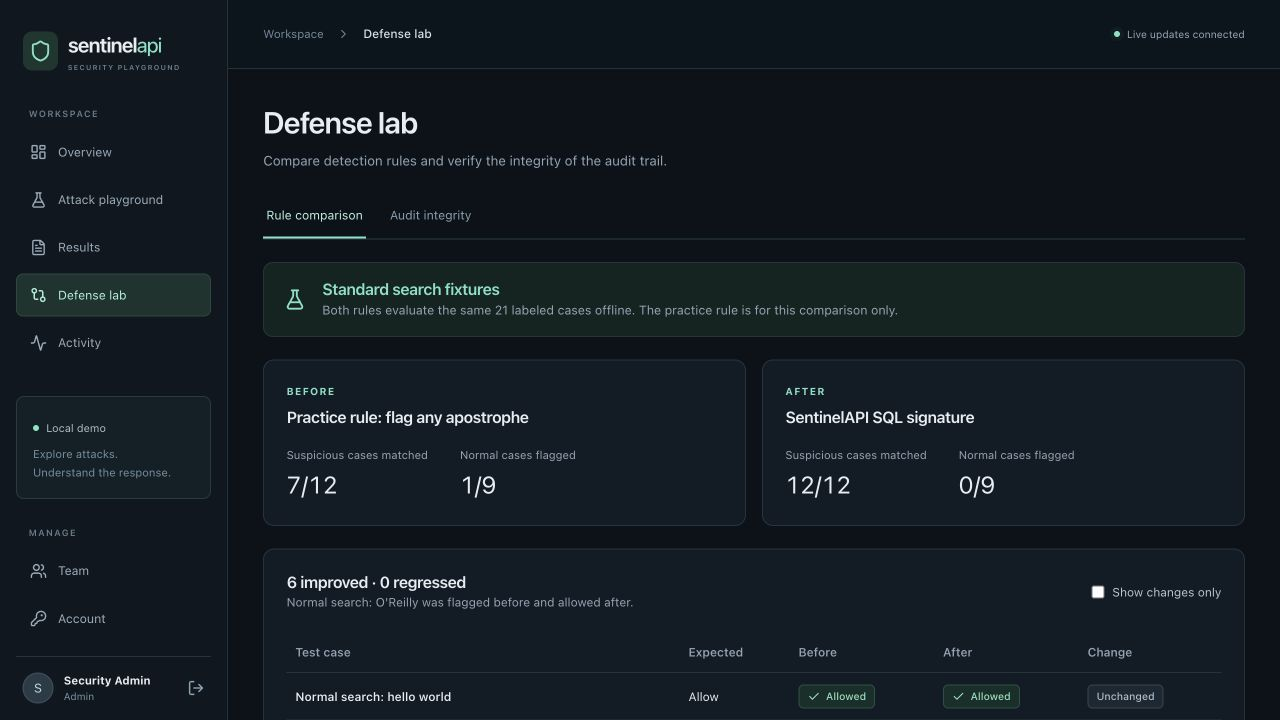
\includegraphics[width=.99\linewidth]{defense-lab.png}
\captionof{figure}{Defense Lab running locally. The screenshot shows the same fixed 21 cases evaluated by the practice rule and the current rule.}
\end{center}

\topic{Navigation used in the demonstration}
The Overview summarizes available experiments. Attack playground presents individual scenarios and controls. Results reopens stored evidence and exports. Defense Lab compares rules and provides the audit verification view for administrators. Activity contains detections, incidents, sign-in history, and the audit trail.

\topic{Challenges and solutions}
Concurrent flood responses can finish in different orders. The verifier uses the persisted trigger evidence for the cooldown check rather than assuming a fixed response order. Old runs lack newly captured explanation fields, so the interface can still display legacy outcomes and alerts. Report formatting also has to keep request text separate from browser markup. The code preserves text, escapes exported HTML, and redacts sensitive values where the evidence format supports it.

\topic{How to use the screenshot}
Read the two result cards together. The baseline matches 7 of 12 suspicious cases and flags 1 of 9 legitimate cases. The current rule matches 12 of 12 and flags 0 of 9. The row for a normal surname is the simplest example to explain why a rule should use context.


\chapter{Testing and Security Evaluation}
\section{Test Design and Expected Results}
The HTTP test oracle checks response status and evidence together. Each scenario states what the API should do and which detector should appear when the case requires an alert. Normal traffic carries a separate expectation that no case-linked alert is present. The recorded HTTP result remains visible even if the case fails its expected detector check.

\tabletitle{Standard profile case distribution}
\begin{tabularx}{\linewidth}{@{}p{.26\linewidth}rX@{}}\toprule
\textbf{Scenario} & \textbf{Cases} & \textbf{Expected behavior}\\\midrule
Normal controls & 12 & 200, no alerts.\\
SQL injection & 12 & 403, SQL Injection evidence.\\
Cross-site scripting & 10 & 403, XSS evidence.\\
Path traversal & 6 & 403, Path Traversal evidence.\\
Command injection & 10 & 403, Command Injection evidence.\\
Password guessing & 20 & Early 401 responses, then 403 plus detector evidence.\\
Password spraying & 10 & Early 401 responses, then 403 plus detector evidence.\\
SSRF indicators & 8 & 403, restricted-host evidence.\\
Disguised upload & 4 & 403, file signature evidence.\\
Scanner headers & 6 & 403, scanner signature evidence.\\
Endpoint enumeration & 15 & 404, with a detector alert at 15.\\
Flood and recovery & 62 & 200/429 during the sequence, 200 on recovery.\\
\midrule
\textbf{Total} & \textbf{175} & \textbf{Response and case-linked evidence compared with the plan.}\\
\bottomrule\end{tabularx}

\topic{Negative controls}
Controls include normal search terms, apostrophes in names, nested but routine JSON, an ordinary upload, a valid demo login, and a public destination in simulated fetch. These cases make false positives measurable within the defined test set. The normal controls have their own profile selection for a quick local confidence check.

\sheet{Functional Testing and Authorization}
Functional testing checks that the application remains usable while the security controls operate. A dashboard screen can appear healthy even if the API is not linked to the database, so a practical check includes startup, status, persisted reports, and a fresh read of an investigation action.

\tabletitle{Functional acceptance cases}
\bodytable{\textbf{Case} & \textbf{Expected observation}\\\midrule
Dashboard startup & Local interface loads and API health reports a connected database.\\
Account login & A valid account can open the dashboard. Invalid credentials return 401.\\
Viewer starts a run & Server refuses the action.\\
Report ownership & An analyst cannot retrieve another user's private report.\\
Alert review & Updating the verdict persists the value and creates an audit event.\\
Incident retrieval & Authorized user sees linked events. An unrelated analyst cannot read the incident.\\
Export & A saved experiment can produce a readable HTML, CSV, or JSON artifact.\\
Audit demo & Original sample verifies. An edited or truncated sample fails.\\}

\topic{Verification method}
The API and database checks used a schema separate from ordinary project history and synthetic evidence for review tests. This let the checks exercise owner, unrelated analyst, viewer, and administrator paths without changing an existing real alert. The verifier also read a deliberately altered database record and a deliberately truncated history.

\topic{What was freshly checked}
The latest verification observed persisted verdicts, separate alert state, account scoping, a role-restricted integrity endpoint, and the audit event shown by the incident timeline. Frontend checks opened the comparison, audit demonstration, and a saved incident. A subsequent normal-case run generated signed application audit events in the ordinary local database.

\sheet{Security Testing and Integrity Checks}
Automated checks cover request normalization, expiration windows, detector isolation, and output handling. The new Defense Lab checks focus on regressions that would be difficult to detect by merely opening the page.

\tabletitle{Security properties and why they are tested}
\bodytable{\textbf{Property} & \textbf{Verification idea}\\\midrule
Normalization & Recognized data inside supported encodings or a nested field reaches the appropriate rule.\\
Normal quotes & An ordinary apostrophe in a name remains accepted by the specific rule.\\
Counter boundary & Compare measures below the threshold and at the threshold. Confirm that the explanation uses the actual count.\\
Authorization & A viewer cannot label an alert. An unrelated analyst cannot cross the ownership boundary.\\
Evidence safety & Matched sensitive fields are redacted and exported values are encoded.\\
Audit changes & Verify an authentic sequence, then edit an old entry and remove the last entry in disposable data.\\}

\begin{lstlisting}[caption={Audit sample assertions based on tests/defense.test.ts}]
for (const change of ['edit', 'delete'] as const) {
  const result = demonstrateAuditIntegrity(change);
  assert.equal(result.original.valid, true);
  assert.equal(result.altered.valid, false);
}
\end{lstlisting}

A historical event outside the signed range remains visible but is excluded from the integrity claim. A previously exported report may also lack structured decision fields. The user can inspect current explanations by selecting a newer saved run. This lets the project extend the schema without inventing facts about older requests.

\sheet{Performance Evaluation}
The reports contain a recorded latency for each completed request. This measures the observed request-response path in the local runner, including application processing and database work that occurs before the response. The report duration is a separate interval that includes orchestration overhead and can include deliberate delays.

\tabletitle{Descriptive timing from archived reports}
\begin{tabularx}{\linewidth}{@{}Xrrrr@{}}\toprule
\textbf{Run} & \textbf{Median} & \textbf{P95} & \textbf{Max} & \textbf{Run time}\\\midrule
Standard, 175 cases & 2 ms & 6 ms & 13 ms & 31.569 s\\
Extended SQL and XSS, 142 cases & 2 ms & 2 ms & 3 ms & 0.398 s\\
Normal traffic, 12 cases & 3 ms & 12 ms & 12 ms & 0.065 s\\
\bottomrule\end{tabularx}

The percentiles use the nearest-rank method on latencies from the saved JSON artifacts. The values summarize individual archived runs and are sensitive to execution conditions. The Standard report contains a 31-second recovery wait, while the selected Extended run covers only two signature families. Comparing their elapsed times does not isolate the cost of any single rule.

\topic{Overhead that matters}
Authentication, parsing, regular-expression checks, counters, database writes, evidence verification, and browser updates each contribute work. Polling and run updates also affect the application experience. The timer values available in the report do not decompose these costs. Guided execution is intentionally slower for teaching.

\topic{A fair follow-up benchmark}
A follow-up should keep corpus, machine, database, concurrency, and runtime constant. It could compare baseline request handling with inspection and persistence using a bounded normal workload. Report repeated runs and variation, separating per-request latency from cooldown and teaching delays. Such data would support a performance claim beyond the current single-run summaries.

\sheet{Evaluation Metrics and Test Protocol}
\topic{Expectation agreement}
Let $n$ be the number of completed cases eligible for comparison and $m$ the number satisfying the declared response and evidence rules.
\[
 \operatorname{Agreement} = \frac{m}{n}.
\]
This metric gives equal weight to each planned check. Some checks are linked, such as the attempts leading to a threshold and the subsequent recovery observation.

\topic{Classification metrics for labeled fixtures}
For the offline comparison, let TP be a suspicious case flagged, FP a normal case flagged, FN a suspicious case allowed, and TN a normal case allowed. Appropriate fixture metrics include
\[
 \operatorname{Recall}=\frac{\mathrm{TP}}{\mathrm{TP}+\mathrm{FN}},
 \qquad
 \operatorname{FPR}=\frac{\mathrm{FP}}{\mathrm{FP}+\mathrm{TN}}.
\]
An empty denominator gives an undefined rate. The offline corpus contains both positive and negative labels. It may overlap the patterns for which the rule was written, so the comparison is a regression exercise rather than an independent estimate.

\topic{Attribution gaps}
For Extended cases, the expected detector provides a reference label. A missing expected detector may occur when a case is allowed or when a different detector responds. The report keeps failed expectations, status counts, and connection errors separate, so a different 403 cannot be misread as proof that the intended detector worked.

\topic{Procedure followed}
Verify builds and unit tests, identify exact saved run artifacts, and compare profile counts and outcomes. Inspect the comparison view and audit demonstration. Check ownership and state transitions in a separate local database schema. Interpret the results in terms of the test set and preserve unexpected cases for review.

\chapter{Results}
\section{Standard Run and Observed HTTP Outcomes}
The archived Standard run with ID prefix \texttt{509674dd} completed all 175 cases. All cases met their configured expectations \cite{artifacts}. The table shows the actual status distribution, which gives more detail than the single agreement figure.

\tabletitle{Observed response distribution in the Standard run}
\begin{tabularx}{\linewidth}{@{}lrX@{}}\toprule
\textbf{Status} & \textbf{Count} & \textbf{Interpretation in the evaluated suite}\\\midrule
200 & 62 & Normal controls and rate-test responses accepted before limiting or after recovery.\\
401 & 8 & Initial incorrect demo logins across the guessing and spraying cases.\\
403 & 78 & Rejections from signature or behavioral detector rules.\\
404 & 15 & Missing routes. An enumeration alert was expected at the threshold.\\
429 & 12 & Rate-limited replies in the local flood experiment, including the cooldown check.\\
\midrule
Total & 175 & 175 expectations matched.\\
\bottomrule\end{tabularx}

The 12 normal controls returned 200 without detector alerts. The successful result for enumeration includes continued 404 responses. An initial 401 in the login sequence is also a correct outcome. Each case is assessed against its own plan, so neither the number of blocks nor the number of successful responses directly measures agreement.

\begin{lstlisting}[caption={An illustrative normal search used to explain the comparison}]
GET /search?q=O%27Reilly
Expected response: 200
Expected detector evidence: no alert
\end{lstlisting}

\topic{Provenance}
The Standard artifact was saved on 2 November 2026 in India Standard Time. It predates the Defense Lab update. Existing records can still be opened using saved evidence. Newly captured rule identifiers and counters are available from runs made after that update.

\topic{Reading the rate-limit result}
A 429 during the designed burst shows temporary limiting within the local scope. A 200 after the planned wait checks recovery. These observations support the application behavior demonstrated by the fixture. They give no performance measurement for traffic from many hosts.

\sheet{Extended Results and Detector Attribution}
The saved Extended run with ID prefix \texttt{c9ed9c0c} selected SQL injection and XSS. It included 142 requests. The two families showed different levels of agreement on the larger set.

\tabletitle{Observed agreement by family in the selected Extended run}
\begin{tabularx}{\linewidth}{@{}Xrrrr@{}}\toprule
\textbf{Scenario} & \textbf{Cases} & \textbf{Matched} & \textbf{Unexpected} & \textbf{Agreement}\\\midrule
SQL injection & 72 & 40 & 32 & 55.6\%\\
Cross-site scripting & 70 & 66 & 4 & 94.3\%\\
\midrule
\textbf{Total} & \textbf{142} & \textbf{106} & \textbf{36} & \textbf{74.6\%}\\
\bottomrule\end{tabularx}

The recorded run contained 34 HTTP~200 and 108 HTTP~403 responses. Although 108 requests were refused, 106 expectations matched. A refusal by a different detector can leave the originally expected rule unobserved. The saved report records 36 missing expected detector attributions and zero transport errors.

\topic{Interpreting coverage}
A broader corpus changes the shape of the evaluation. Inputs may require a specific insertion point, context, or interpreter to have security significance. Some simply do not match the project's fixed signatures. SentinelAPI preserves unexpected results so the team can discuss why reviewed examples should be added to a future regression set. The lab handlers keep submitted data inert.

\topic{Limit of the result}
The 142-row artifact was saved on 26 October 2026. The planned full Extended suite contains 295 cases. The 74.6\% figure describes the selected two-family experiment and does not apply to the unmeasured full Extended plan.

\sheet{Before and After Rule Comparison}
The comparison uses 21 labeled search cases, comprising 12 suspicious cases and 9 normal cases. The practice rule flags any apostrophe. The application rule looks for more specific SQL signatures. Both rules receive the same extracted values.

\tabletitle{Confusion counts on the fixed comparison set}
\begin{tabularx}{\linewidth}{@{}Xrr@{}}\toprule
\textbf{Outcome} & \textbf{Practice rule} & \textbf{Application rule}\\\midrule
True positives & 7 & 12\\
False negatives & 5 & 0\\
False positives & 1 & 0\\
True negatives & 8 & 9\\
\midrule
Correct fixture decisions & 15/21 & 21/21\\
Suspicious-case recall & 58.3\% & 100.0\%\\
Normal-case false-positive rate & 11.1\% & 0.0\%\\
\bottomrule\end{tabularx}

Six outcomes improved and none regressed on these cases. Five additional suspicious cases were recognized and one normal case stopped being flagged. The normal example is \texttt{O'Reilly}. Its punctuation is ordinary for a surname. The difference is visible in the highlighted result row.

\topic{Why the comparison matters}
A rule change can reduce one type of error and raise another. Evaluating both rules on the same normal and suspicious cases shows both sides of the trade-off. The comparison connects the interface to measurable values rather than relying on the fact that one rule looks more complex.

\topic{Limits of the comparison}
The result describes the labeled fixture set. It does not show equal performance on independent traffic or all SQL contexts. The archived Extended run provides a separate example of why broader evaluation is needed. Future changes can reuse the same acceptance set and add independently labeled normal cases.

\sheet{Investigation, Audit and Verification Evidence}
\tabletitle{Verification performed after the Defense Lab update}
\bodytable{\textbf{Check} & \textbf{Observed result}\\\midrule
Backend and UI quality checks & Build and lint passed. All 12 automated tests passed.\\
New normal-traffic run & \texttt{a9fce53e}: all 12 cases returned 200 with no alert.\\
Review persistence & The isolated test saved a false-positive verdict, read it back, and checked its audit event.\\
Account access & Viewer write and out-of-scope analyst access were refused. Authorized access worked in the isolated test.\\
Live audit trail & Two newly signed events verified in the ordinary project database.\\
Tamper detection & An edit and a removed final event each failed verification in disposable data.\\}

\topic{Evidence an assessor can inspect}
A run identifier links the timeline, the actual response, and any recorded detector. Selecting an alert shows its detector name and review status. The analyst can confirm or reject the finding and then inspect the incident timeline to see when that decision occurred. The audit verifier gives an independent integrity check of signed events.

\topic{What the results support}
The system demonstrated local rule evaluation, controlled response behavior, and persistent investigation actions. Role checks separated administrative actions from owned evidence and ordinary review. The integrity results confirm that the verifier distinguishes the original signed sample from the tested modifications. Each claim is tied to the run, fixed dataset, or isolated check that measured it.

\chapter{Conclusion and Future Work}
\section{Conclusion and Demonstration Sequence}
SentinelAPI combines request signatures and scoped behavioral counts and connects the results to persistent alert evidence. Operators can see why the status changed, compare rules on a fixed set, revisit a saved result, and record a judgment. The system demonstrates how prevention, detection, and investigation complement one another.

The archived Standard suite matched all 175 expectations. The broader selected Extended suite produced 36 attribution gaps. The before-and-after comparison showed how a more specific rule removed one false positive and recognized five additional suspicious fixtures. The newer normal-traffic run confirmed ordinary request behavior after the investigation features were added.

\topic{Suggested classroom demonstration}
\begin{enumerate}
\item Open Defense Lab and use Show changes only. Explain the ordinary surname example.
\item Open a recent result and select Explain this decision. For a behavioral case, compare measurements below and at a threshold.
\item Open a saved incident and inspect linked alerts and investigator actions.
\item Show how recording a review verdict differs from resolving the alert.
\item Verify newly signed audit records, then run the disposable edit or deletion demonstration.
\end{enumerate}

\topic{Information security contribution}
The project gives students concrete examples of confidentiality-related request patterns, availability controls, authenticated access, and accountability. The audit chain adds an integrity example whose outcome can be observed directly. The investigation view also shows how security outcomes and human judgments can remain visible independently of each other.

\sheet{Limitations and Future Work}
\topic{Detection coverage}
The rules cover selected signatures and contexts. A raw probe can require a specific interpreter or application behavior that is absent in this lab. An extension would build an independently labeled set of normal and suspicious API examples and track errors over successive policy revisions. The rule comparison could store immutable test-set versions to make historical evaluations easier to reproduce.

\topic{Deployment and measurement}
In-memory counters are appropriate for a single process. A future multi-instance service would need shared counter state and consistent request identity. A separate deployment review could evaluate access policies, browser security headers, and configuration changes. Benchmarks could evaluate ordinary load, concurrent operators, and database-write behavior on a fixed machine with repeated runs.

\topic{Evidence integrity}
Current integrity verification depends on a protected key and a trustworthy checkpoint. The signed range starts after the feature was installed. Periodically keeping a checkpoint in independent, write-restricted storage would help detect rollback of the database together with its embedded checkpoint. A key-rotation plan should preserve the history needed to verify earlier signed events.

\topic{Investigation workflow}
Incident grouping uses known experiment relationships. An extension could group hand-reviewed signals over time and record analyst notes. Review totals could display agreement between reviewers and separate experimental fixtures from ordinary interface activity. Those measures would help explain how investigation workload changes as rules evolve.

\topic{Next evaluation milestone}
Repeat Standard and Extended tests on the version submitted, retain their reports, and record the runtime configuration used. Expand normal-traffic controls before claiming better general-purpose accuracy.

\renewcommand{\bibname}{References}
\begin{thebibliography}{9}
\addcontentsline{toc}{chapter}{References}
\small
\setlength{\itemsep}{.5em}
\bibitem{nist} K. Scarfone and P. Mell, \emph{Guide to Intrusion Detection and Prevention Systems (IDPS)}, NIST SP 800-94, 2007. \url{https://doi.org/10.6028/NIST.SP.800-94}.
\bibitem{owasp} OWASP Foundation, \emph{Web Security Testing Guide}, v4.2. \url{https://wstg.owasp.org/v4.2/4-Web_Application_Security_Testing/}.
\bibitem{bozic} J. Bozic and F. Wotawa, \emph{Planning-based security testing of web applications with attack grammars}, Software Quality Journal, vol. 28, pp. 307--334, 2020. \url{https://doi.org/10.1007/s11219-019-09469-y}.
\bibitem{hmac} H. Krawczyk, M. Bellare and R. Canetti, \emph{HMAC: Keyed-Hashing for Message Authentication}, RFC 2104, 1997. \url{https://www.rfc-editor.org/info/rfc2104}.
\bibitem{http} R. Fielding, M. Nottingham and J. Reschke, eds., \emph{HTTP Semantics}, RFC 9110, 2022. \url{https://www.rfc-editor.org/info/rfc9110}.
\bibitem{rfc429} M. Nottingham and R. Fielding, \emph{Additional HTTP Status Codes}, RFC 6585, 2012. \url{https://www.rfc-editor.org/info/rfc6585}.
\bibitem{jwt} M. Jones, J. Bradley and N. Sakimura, \emph{JSON Web Token (JWT)}, RFC 7519, 2015. \url{https://www.rfc-editor.org/info/rfc7519}.
\bibitem{seclists} D. Miessler and contributors, \emph{SecLists}, repository and license. \url{https://github.com/danielmiessler/SecLists}. Pinned revision cited in Chapter 4.
\bibitem{artifacts} SentinelAPI project repository. Local implementation and archived run artifacts, including Standard run \nolinkurl{509674dd-9714-43ec-a701-b1db316f19c1}, Extended run \nolinkurl{c9ed9c0c-afd0-41d5-af37-91721ba5302b}, and normal run \nolinkurl{a9fce53e-f017-4148-bdf6-f37850cee805}. Defense Lab verification recorded in November 2026.
\end{thebibliography}
\end{document}

